\documentclass[10pt]{beamer}

\usepackage{amssymb,amsfonts,amsmath,mathtext}
\usepackage[T2A]{fontenc}
\usepackage[utf8]{inputenc}
\usepackage[english,russian]{babel}
\usepackage{cite,enumerate,float,indentfirst}
\usepackage{graphicx}

%For putting links into papers, also helps make cross-references in the paper smart references
% \usepackage[colorlinks = true, linkcolor = blue, urlcolor  = blue, citecolor = blue, anchorcolor = blue]{hyperref} 
%smarter cross-references, these options turn links blue

%Tables
\usepackage{caption} %For table captions

%highlights text with \hl{text}
\usepackage{color, soul}

\graphicspath{{images/}}
\DeclareGraphicsExtensions{.pdf,.png,.jpg}
% \usepackage{palatino}
\usepackage{graphicx}
\usepackage{colortbl}
\usepackage{xcolor}
\usepackage{ifthen}
\usepackage{subfigure}
\usepackage{amsthm}
\usepackage{chngcntr}
\counterwithin{figure}{section}

\RequirePackage{caption}
% \DeclareCaptionLabelSeparator{defffis}{ -- } % Separator

\captionsetup[figure]{
    justification=centering,
    labelfont=it,
    textfont={bf,it},
    labelsep=colon,
    format=plain} % Подпись рисунка по центру

\captionsetup[table]{
    justification=raggedright,
    labelfont=it,
    textfont={bf,it},
    labelsep=colon,   
	format=plain, 
	singlelinecheck=false
} % Подпись таблицы слева

\mode<presentation> {
  %\usetheme{Warsaw}
  \usetheme{Madrid}
  %\usetheme{Frankfurt}
  \usecolortheme{seahorse}
}

\addtobeamertemplate{frametitle}{}{%     upper-line
	\vskip-1em
}

\title[]{\large{Построение матрицы влияния для планарной трещины в слоистой области. Быстрое умножение однородной матрицы влияния на вектор раскрытия}}
\author[Абдуллин Р.Ф]{Абдуллин Рустам Фаритович \\[1cm]
{\emph{Научный руководитель:} д-р физ.-мат. наук, проф. РАН \mbox{Головин Сергей Валерьевич}}}

\institute[НГУ]
{
\vspace{0.5cm}
\begin{minipage}{0.5\linewidth}
  \begin{center}
  	\textbf{ НОВОСИБИРСКИЙ ГОСУДАРСТВЕННЫЙ УНИВЕРСИТЕТ, НГУ}
  \end{center}
\end{minipage}
}

% \date{7 ноября 2019}
\setbeamertemplate{navigation symbols}{}


\begin{document}
\begin{frame}
\titlepage 
\end{frame}


\begin{frame}
	\frametitle{Материалы}
	\begin{itemize}
		\item \footnotesize{A. P. Peirce and E. Siebrits, "Uniform asymptotic approximations 
		for accurate modeling of cracks in layered elastic media", International Journal of Fracture",
		110, 205-239, 2001.}
		\item \footnotesize{A.P. Peirce and E. Siebrits,
		"The scaled flexibility matrix method for the efficient solution of boundary value problems
		in 2D and 3D layered elastic media", Computer Methods in Applied Mechanics and Engineering}
		\item \footnotesize{E. Dontsov, MATLAB code}
	\end{itemize}
	
\end{frame}


\begin{frame}
\frametitle{Постановка задачи}
\begin{columns}
	\begin{column}{0.35\textwidth}
	    \begin{figure}
	    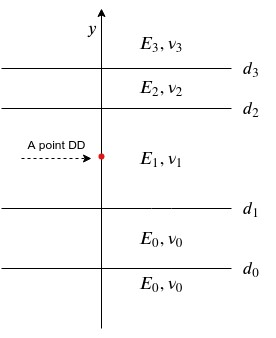
\includegraphics[width=\textwidth]{DDPoint}
	    \caption{\footnotesize Геометрия слоистого тела}     
	    \end{figure}
	\end{column}

	\begin{column}{0.35\textwidth}
	    \begin{figure}
	    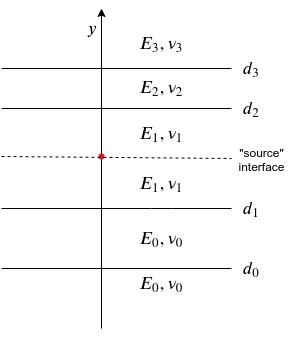
\includegraphics[width=\textwidth]{pseudointerface}
	    \caption{\footnotesize Добавление псевдо-границы}     
	    \end{figure}
	\end{column}
\end{columns}
\end{frame}



\begin{frame}
\frametitle{Определяющие уравнения}
Уравнения упругой изотропной среды задаются формулами:
\begin{equation}
	\label{eq:equilibrium}
	\sigma_{ij,j} + f_j = 0,
\end{equation}
\begin{equation}		
	\label{eq:hooke}
	\sigma_{ij} = \lambda e_{kk}\delta_{ij} + 2G e_{ij},
\end{equation}
где $\lambda = \frac{E \nu}{(1+\nu)(1-2\nu)}$ и $ G = \frac{E}{2(1+\nu)} $.
\end{frame}



\begin{frame}
\frametitle{Определяющие уравнения}
Отделим производные по $y$ от производных по $x, y$ в (\ref{eq:equilibrium}) и (\ref{eq:hooke}):
\begin{equation}
	\label{eq:separate}
	\partial_{y} T = \mathbb{A}T,
\end{equation}

где $T$ -- вектор
\begin{equation}
	\label{eq:T}
	T = \left[\sigma_{yy} \; \sigma_{xy} \; \sigma_{yz} \; u_{y} \; u_{x} \; u_{z}\right]^T,
\end{equation}

и $\mathbb{A}$ -- дифференциальный оператор, который содержит производные только по $x$ и $z$
\begin{equation}
	\label{eq:A}
	\mathbb{A} = 
	\left[\begin{array}{cccccc}
		0 & -\partial_x & -\partial_z & 0 & 0 & 0 \\
		-\frac{b}{a}\partial_x & 0 & 0 & 0 & \frac{b^2-a^2}{a}\partial_{xx} - \frac{f}{2}\partial_{zz} & \left( \frac{b^2-ab}{a} - \frac{f}{2} \right) \partial_{xz} \\
		-\frac{b}{a}\partial_z & 0 & 0 & 0 & \left( \frac{b^2-ab}{a} - \frac{f}{2} \right) \partial_{xz} & \frac{b^2-a^2}{a}\partial_{zz} - \frac{f}{2}\partial_{xx} \\
		\frac{1}{a} & 0 & 0 & 0 & -\frac{b}{a}\partial_x & -\frac{b}{a}\partial_z \\
		0 & \frac{2}{f} & 0 & -\partial_x & 0 & 0 \\
		0 & 0 & \frac{2}{f} & -\partial_z & 0 & 0 
	\end{array}\right],
\end{equation}
\end{frame}



\begin{frame}
\frametitle{Определяющие уравнения}
где используются константы
\begin{align*}
	a & = \lambda + 2G, &     b & = \lambda, &     f & = 2G, \\
	l_2 & = \frac{\lambda + 3G}{\lambda + G}, &     l_4 & = \frac{2G^2}{\lambda+G}, &   l_5 & = \frac{2G(\lambda + 2G)}{\lambda + G}, \\
	l_6 & = \frac{2G(2\lambda + 2G)}{\lambda + G}, &   l_7 & = \frac{2\lambda G}{\lambda+G}
\end{align*}
\end{frame}


\begin{frame}
\frametitle{Преобразование Фурье}
Применим преобразование Фурье (2D) для (\ref{eq:separate}) по координатам $x$ и $z$
\begin{equation}
	\label{eq:FourierTransform}
	\partial_y \hat{T} = \hat{\mathbb{A}} \hat{T},
\end{equation}
где
\begin{equation}
	\label{eq:FourierT}
	\hat{T} = \left[\hat{\sigma}_{yy}/k \quad \hat{\tau}_s/k \quad \hat{u}_y \quad \hat{u}_s \quad  \hat{\tau}_t/k \quad  \hat{u}_t \right]^T,
\end{equation}
и оператор $\hat{\mathbb{A}}$:
\begin{equation}
	\label{eq:FourierA}
	\hat{\mathbb{A}} = 
	\left[\begin{array}{cccccc}
		0 & -k & 0 & 0 & 0 & 0 \\
		\frac{b}{a}k & 0 & 0 & -\frac{b^2-a^2}{a}k^2 & 0 & 0 \\
		\frac{1}{a} & 0 & 0 & -\frac{b}{a}k & 0 & 0 \\
		0 & \frac{2}{f} & k & 0 & 0 & 0 \\
		0 & 0 & 0 & 0 & 0 & \frac{f}{2}k \\
		0 & 0 & 0 & 0 & \frac{2}{f} & 0 
	\end{array}\right],
\end{equation}
\end{frame}



\begin{frame}
\frametitle{Преобразование Фурье}
Компоненты перемещения
\begin{equation}
	\label{eq:FourierDisplacment}
	\begin{split}
	\hat{u}_s & = -i \left( m\hat{u}_x + n\hat{u}_z \right) / k, \\
	\hat{u}_t & = -i \left( n\hat{u}_x - m\hat{u}_z \right) / k,
	\end{split}
\end{equation}

и компоненты напряжения
\begin{equation}
	\label{eq:FourierDisplacment}
	\begin{split}
	\hat{\tau}_s & = -i \left( m\hat{\sigma}_{xy} + n\hat{\sigma}_{yz} \right) / k, \\
	\hat{\tau}_t & = -i \left( n\hat{\sigma}_{xy} - m\hat{\sigma}_{yz} \right) / k,
	\end{split}
\end{equation}


Здесь $m$ и $n$ координаты в пространстве Фурье, взаимные с $x$ и $z$ соответственно, $k = \sqrt{m^2+n^2} $
\end{frame}



\begin{frame}
\frametitle{Решение ОДУ}
Решение системы (\ref{eq:FourierTransform}):
\begin{equation}
	\label{eq:FourierSolution}
	\left[
	\begin{array}{c}
		\hat{T}_s \\
		\hat{T}_t 
	\end{array}
	\right]
	=
	\left[
	\begin{array}{cc}
		Z_s & 0 \\
		0 & Z_t 
	\end{array}
	\right]
	\left[
	\begin{array}{c}
		A_s \\
		A_t 
	\end{array}
	\right]
\end{equation}

где используются обозначения:
\begin{equation}
	\label{eq:FourierSeparateT}
	\hat{T}_s = \left[\hat{\sigma}_{yy}/k \quad \hat{\tau}_s/k \quad \hat{u}_y \quad \hat{u}_s \right]^T, \qquad 
	\hat{T}_t = \left[ \hat{\tau}_t/k \quad  \hat{u}_t \right]^T,
\end{equation}

и спектральные коэффициенты:
\begin{equation}
	\label{eq:FourierSeparateA}
	A_s = \left[ A_1 \quad A_2 \quad A_3 \quad A_4 \right]^T, \qquad 
	A_t= \left[ A_5 \quad A_6 \right]^T.
\end{equation}
\end{frame}



\begin{frame}
\frametitle{Решение ОДУ}
Матрицы $Z_s$ и $Z_t$ имеют вид:
\begin{equation}
	\label{eq:FourierSeparateA}
	\begin{split}
	Z_s & = 
	\left[
	\begin{array}{cccc}
		-fe^{-ky} & (l_4-fky)e^{-ky} & fe^{ky} & (l_4+fky)e^{ky} \\
		-fe^{-ky} & (l_5-fky)e^{-ky} & -fe^{ky} & -(l_5+fky)e^{ky} \\
		e^{-ky} & kye^{-ky} & e^{ky} & kye^{ky} \\
		e^{-ky} & (ky-l_2)e^{-ky} & -e^{ky} & -(ky+l_2)e^{ky} \\
	\end{array}
	\right],
	\\
	Z_t & = 
	\left[
	\begin{array}{cc}
		-\frac{f}{2}e^{-ky} & \frac{f}{2}e^{ky} \\
		e^{-ky} & e^{ky}
	\end{array}
	\right].
	\end{split}
\end{equation}
\end{frame}



\begin{frame}
\frametitle{Спектральные коэффициенты}
\begin{equation}
	\label{eq:AS}
	\left[
	\begin{array}{c}
	A^{j}_{1}(k) \\
	A^{j}_{2}(k)\\
	A^{j}_{3}(k) \\
	A^{j}_{4}(k)
	\end{array}
	\right]
	= \frac{1}{2l^j_5}
	\left[
	\begin{array}{cccc}
		-l^j_2 & 0 & l^j_5 & -l^j_4 \\
		-1 & 1 & f^j & -f^j \\
		l^j_2 & 0 & l^j_5 & l^j_4 \\
		-1 & -1 & -f^j & -f^j
	\end{array}
	\right]
	\left[
	\begin{array}{c}
	\hat{\sigma}^{j}_{yy}(y=y_j)/k \\
	\hat{\tau}^{j}_{s}(y=y_j)/k\\
	\hat{u}^{j}_{y}(y=y_j) \\
	\hat{u}^{j}_{s}(y=y_j) 
	\end{array}
	\right],
\end{equation}

\begin{equation}
	\label{eq:At}
	\left[
	\begin{array}{c}
	A^{j}_{5}(k) \\
	A^{j}_{6}(k)
	\end{array}
	\right]
	= \frac{1}{2l^j_5}
	\left[
	\begin{array}{cc}
		-\frac{1}{f^j} & \frac{1}{2} \\
		\frac{1}{f^j} & \frac{1}{2}
	\end{array}
	\right]
	\left[
	\begin{array}{c}
	\hat{\tau}^{j}_{t}(y=y_j)/k\\
	\hat{u}^{j}_{t}(y=y_j) 
	\end{array}
	\right].
\end{equation}

Когда спектральные коэффициенты для слоя найдены, используя (\ref{eq:FourierSolution}) и соотношение (\ref{eq:hooke}), получим:
\begin{multline}
	\hat{\sigma}^j_{zz}(y)/k = f\frac{n^2}{k^2}e^{-ky}A^j_1(k)
	- \left(l_6\frac{n^2}{k^2}+l_7\frac{m^2}{k^2}-f\frac{n^2}{k^2}ky \right)e^{-ky}A^j_2(k) \\
	- f\frac{n^2}{k^2}e^{ky}A^j_3(k)
	- \left(l_6\frac{n^2}{k^2}+l_7\frac{m^2}{k^2}+f\frac{n^2}{k^2}ky \right)e^{ky}A^j_4(k) \\
	- f\frac{mn}{k^2}e^{-ky}A^j_5(k)
	- f\frac{mn}{k^2}e^{ky}A^j_6(k).
\end{multline}
\end{frame}


\begin{frame}
	\frametitle{}
	Условие $u_{z-0} - u_{z+0} = \Delta u$ может быть представлено в виде:

	\begin{equation}
		\label{eq:JumpCondition}
		\left[ \hat{T} \right] = 
		\left[ \begin{array}{c} 
			0 \\ \frac{\Delta u(b^2 - a^2)}{a} \\ \frac{\Delta ub}{a} \\ 0 \\ 0 \\ 0 
		\end{array} \right]
		+
		\frac{m^2}{m^2+n^2} \left[ \begin{array}{c} 
			0 \\ \Delta u(a-b) \\ 0 \\ 0 \\ 0 \\ 0 
		\end{array} \right]
		+
		\frac{mn}{m^2+n^2} \left[ \begin{array}{c} 
			0 \\ 0 \\ 0 \\ 0 \\ \Delta u(a-b) \\ 0 
		\end{array} \right]	
	\end{equation}

	Связывание решений на каждом слое:
	\begin{equation}
		A^i p^{i-1} + C^i p^i + B^i p^{i+1} = D^i
	\end{equation}
	
\end{frame}




\begin{frame}
\frametitle{Связь с давлением жидкости внутри трещины}
Условие для точечного DD является сингулярным, поэтому решение будем искать в виде 
разницы полного решения и решения для однородной среды \textit{(которое можно получить аналитически)}:
\begin{equation}
	\Delta \hat{\sigma}_{zz} = \hat{\sigma}_{zz} - \hat{\sigma}_{zz,0}
\end{equation}

Таким образом, для расчёта давления жидкости внутри трещины:
\begin{equation}
	\label{eq:fluidPressure}
	\begin{split}
	p(x,y) = & \sigma_h(y)-\frac{E'(y)}{8\pi}\int \frac{w(x',y')dx'dy'}{\left[(x-x')^2+(y-y')^2\right]^{3/2}} \\
	- & \int \Delta\sigma_{zz}(x,y,x',y')w(x',y')dx'dy'
	\end{split}
\end{equation}
где $\sigma_h(y)$ -- горизонтальные напряжения в пласте, $ E'(y) = E(y)/(1-\nu^2) $
\end{frame}


\begin{frame}
	\frametitle{Минусы подхода}
	$X, Y$ -- количество ячеек вдоль осей $x$ и $y$ -- соответственно, $N$ -- количество слоев. Тогда время расчёта:
	\begin{equation}
		T^\text{FFT} = Y\cdot X^2 \left( \underbrace{C_1\cdot N}_{\begin{array}{c}
		\text{вект. прогонка} + \\
		\text{вычисление} \hat{\sigma}_{zz}
		\end{array}} + \underbrace{C_2^\text{FFT}\cdot Y \log X}_{\text{FFT}}\right)
	\end{equation}
	где $\boxed{C_1 \approx 1.9 \times 10^{-6}, C_2 \approx 3.7 \times 10^{-8}}$
	
	\begin{center}
		\begin{tabular}{ |c|c|c|c|c|} 
			\hline
			Case & X & Y & N & t, c.\\ 
			\hline 
			1 & 40 & 40 & 20 & 3.52 \\ \hline
			2 & 100 & 100 & 4 & 32.3 \\ \hline
			3 & 120 & 120 & 40 & 180 \\ 
			\hline
		\end{tabular}
	\end{center}
\end{frame}


\begin{frame}
	\frametitle{Минусы подхода}
	Проблемы при расширении на модель одновременной инициации нескольких Planar3D-х трещин \textit{(MultiPlanar)}:
	\begin{itemize}
		\item Учёт взаимного влияния трещин друг на друга,
		\item при $L > X, Y$ -- нужно увеличивать количество ячеек в сетке при FT,
		\item неприменим при неортогональном расположении трещин.
	\end{itemize}
	\begin{figure}
	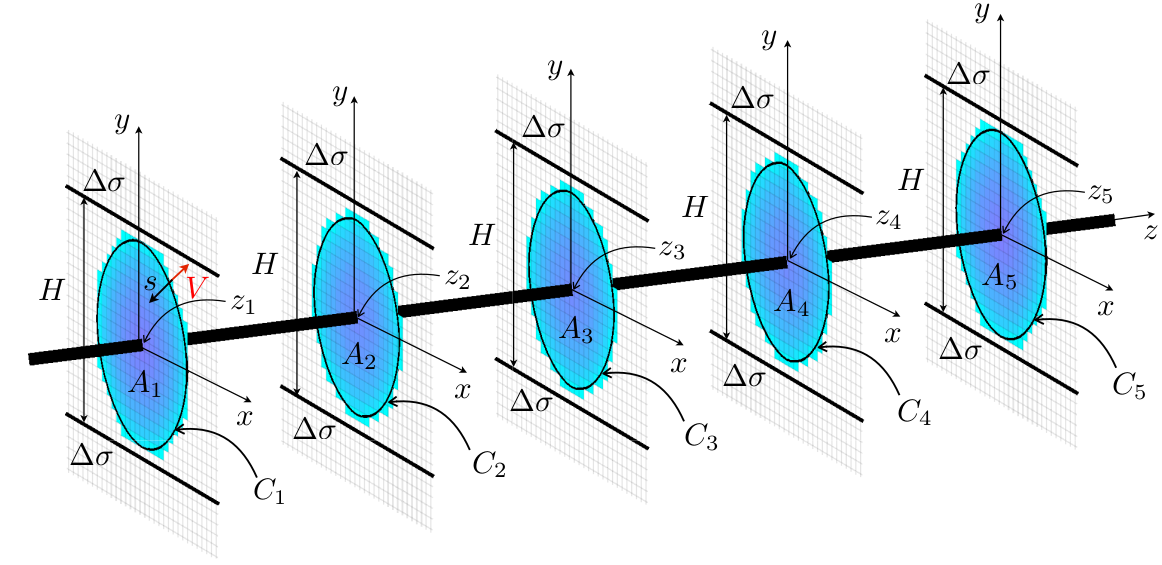
\includegraphics[width=0.8\textwidth]{parallel_planar3d} 
	\end{figure}
\end{frame}

\begin{frame}
	\frametitle{Минусы подхода}
	\begin{figure}
		\includegraphics[width=0.6\hsize]{deviated_horizontal} 
		\caption{Наклонное расположение трещин относительно ствола скважины} 
	\end{figure}
\end{frame}

% \begin{frame}
% 	\begin{equation}
% 	\boxed{
% 	\begin{split}
% 		\sigma_{zz}(x,z) & =\frac{1}{(2\pi)^2} \iint_{\mathbb{R}^2}e^{-i(mx+nz)}\hat{\sigma}_{zz}(m,n) dm \;dn, \\
% 		\hat{\sigma}_{zz}(m,n) & = f_0(k) + f_1(k) \cos 2\theta + f_2(k) \cos 4\theta, \\
% 	\end{split}
% 	}
% 	\end{equation}

% 	\begin{equation}
% 		(-1)^n \int_{-\pi}^{\pi}e^{-ikr\cos(\theta-\phi)} \cos (2n\theta) d\theta = 2\pi J_{2n}(kr)\cos (2n\phi).
% 	\end{equation}
% 	Таким образом, сводим 2D-FT к трем 1D-HT.

% 	\begin{equation}
% 		T^\text{FFT} = Y\cdot X^2 \left( C_1\cdot N + C_2^\text{FFT}\cdot Y \log X\right)
% 	\end{equation}

% 	\begin{equation}
% 		T^\text{HT} = Y\cdot X \left( C_1\cdot N + C_2^\text{HT}\cdot Y \log X\right)
% 	\end{equation}
% \end{frame}



\begin{frame}
	\frametitle{Быстрое умножение матрицы на вектор}
	
	\begin{equation}
		p(\vec{r}) = \frac{E'}{8 \pi} \iint\limits_{\Omega} \frac{w(\vec{r}')}{(\vec{r}-\vec{r}')^3} d\vec{r}'
	\end{equation}

	\begin{equation}
		\begin{split}
			\hat{p}(\vec{k}) & = \iint p(\vec{r}) e^{-i\vec{k}\vec{r}} d\vec{r} = \\
			& = \frac{E'}{8 \pi} \iint \left( \iint\limits_{\Omega} 
			\frac{w(\vec{r}')}{(\vec{r}-\vec{r}')^3} d\vec{r}' \right) e^{-i\vec{k}\vec{r}} d\vec{r} 
			= - \frac{E' \vec{k}}{4} \hat{w} (\vec{k})
		\end{split}
	\end{equation}
	
	При однородной матрице влияния:
	\begin{equation}
		A\cdot w = p,
	\end{equation}

	\begin{equation}
		p_{ij} = \sum \limits_{m=X_b}^{m=X_t} \sum \limits_{n=Y_b}^{n=Y_t} w_{mn} \cdot G_{(i-m), (j-n)}
	\end{equation}

\end{frame}



\begin{frame}
	\frametitle{План работы}
	\begin{itemize}
		\item
		Программная реализация быстрого умножения матрицы на вектор и сопряжение с BISGStab

		\item
		Сопряжение кода расчета матрицы влияния в слоистой среде с Planar3D
	\end{itemize}
	\bigskip
	\begin{center}
		\huge
		Спасибо за внимание!
	\end{center}
\end{frame}


\end{document}